% Lecture for ph2a Caltech 2017: Vibrations and Waves
\documentclass[pdf,hideothersubsections]{beamer}
\usepackage{beamerthemeshadow}
\mode<presentation>
  {
    \usefonttheme{structuresmallcapsserif}
    \usetheme{CambridgeUS}
    \usecolortheme{seahorse}
    %\useinnertheme{circles}
%    \useoutertheme{tree}
  }

\usepackage{svg}
\usepackage{xmpmulti}

\usepackage{hyperref}
\hypersetup{
    pdffitwindow=true,     % window fit to page when opened
    colorlinks=true,       % false: boxed links; true: colored links
    linkcolor=orange,          % color of internal links (change box color with linkbordercolor)
    citecolor=green,        % color of links to bibliography
    filecolor=magenta,      % color of file links
    urlcolor=blue,           % color of external links
   pdfstartview={Fit}
}

% Fonts/encoding
\renewcommand{\UrlFont}{\tiny}
\usepackage[utf8]{inputenc}
\usepackage[T1]{fontenc}
%\usepackage[sc,medium,raggedright]{titlesec}
\usepackage{newtxmath}
%\usepackage{libertine}
\usepackage[osf]{ebgaramond}

\graphicspath{{Figures/}}

\begin{document}
\title{Driven Oscillations and Resonance}  
\author{Caltech: ph2a}
\date{5 - Oct - 2017}
%\logo{
\includegraphics[height=0.5cm]{../caltech_logo.png}}

\frame{\titlepage} 

\frame{\frametitle{Table of contents}\tableofcontents} 

\setbeamerfont{footnote}{size=\tiny}

\section{Previous Summary}
\begin{frame}
\frametitle{Recently}
\begin{itemize}
\item Q is a measure of the 'Quality' of an oscillator; how many cycles it
  takes to ring down: $Q = \omega_0 \tau / 2$
\pause
\item Air track demo shows how this effect works for a driven oscillator
\pause
\item High Q oscillators have a narrow 'bandwidth'. The resonance has
  a sharp peak in the frequency domain.
\pause
\item Undamped SHO energy $= \frac{1}{2}m \dot{x}^2 + \frac{1}{2}k x^2$
\end{itemize}
\end{frame}




\section{Driven Oscillations}
\begin{frame}
\frametitle{Overview}
\pause
\begin{enumerate}
\item For free vibrations, $m \ddot{x} + b \dot{x} + k x = 0$. For a
  driven system the R.H.S. is \emph{not} equal to zero.
\pause
\item For general driven systems, the RHS can be anything: a series of impulses, a few
  cycles of a sine wave, the sum of many sine waves, shark fin wave,
  random noise, etc. Arbitrary forces can be applied to objects.
\pause
\item As we shall see in Lecture \#8, we can usually represent
  arbitrary forces as a sum of sinusoidal forces of differing
  frequencies, phases, and amplitudes.
\pause
\item As a warm up, we consider the case of a harmonically driven,
  damped, simple harmonic oscillator. This simple analysis actually
  solves everything due to a beautiful symmetry between time and frequency.
\end{enumerate}
\end{frame}

\subsection{Solving the Harmonically driven SHO}
\begin{frame}
\frametitle{Setting up the problem}
In the case of a (sinusoidally) driven SHO, the $F$, in $F = m a$, now
has an additonal term:
\pause
\begin{centering}
\begin{align*}
\action<+->{m \ddot{x} &= -k x - b \dot{x} + F(t) \\}
\action<+->{-m \omega^2 x + i \omega b x + k x &= F_0 e^{i (\omega t)} \\}
\action<+->{\frac{A}{F_0} &= \frac{1/m}{\omega_0^2 + i \omega \frac{b}{m} - \omega^2}}
\end{align*}
\end{centering}
\pause
where $A$ is the amplitude of the oscillation ($\tilde{x} = A(\omega) e^{i(\omega t)}$).

\end{frame}

\begin{frame}
\frametitle{The Bode plot: Mag \& Phase vs. Frequency}
\begin{columns}
  \begin{column}{0.5\textwidth}
      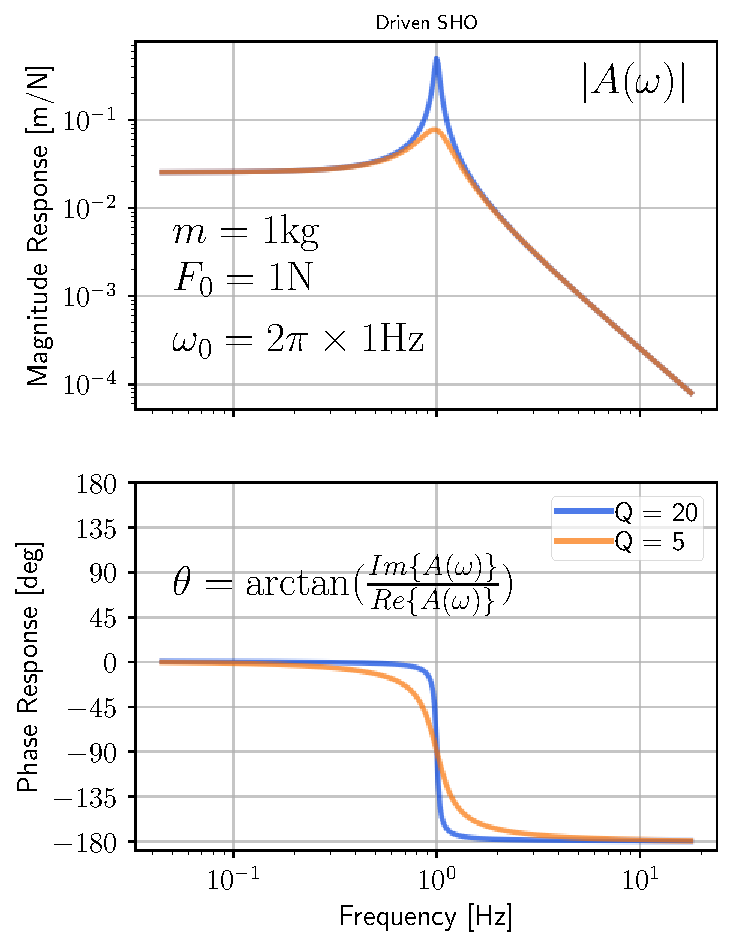
\includegraphics[height=0.8\textheight,keepaspectratio]{DrivenSHO.pdf}
  \end{column}
  \begin{column}{0.5\textwidth}
    \begin{enumerate}
      \pause
      \item The magnitude of the response is the absolute value of the
        ratio of the displacement to the force (independent of phase
        lag).
      \pause
      \item To get the \emph{relative} phase between the force and the
        displacement, we need to use Euler's formula: $e^{i \theta} =
        cos{\theta} + i \sin{\theta}$
        \pause
      \item $\theta$ is in units of \emph{radians}, so we multiple by
        $\frac{180}{\pi}$ to get to \emph{degrees} for this plot
    \end{enumerate}
  \end{column}

\end{columns}
\end{frame}


\subsection{Quality Factor}
\begin{frame}
\frametitle{The Quality Factor: I}
\pause
\begin{block}{Definition I:}
$Q \equiv 2 \pi \frac{\rm energy~stored}{\rm energy~dissipated~per~cycle}$
\end{block}
\pause
\begin{block}{Definition II:}
$Q \simeq \omega_0 \tau / 2$ \\
-- accurate for high Q\footnotemark systems
\end{block}

\footnotetext[1]{Not to be confused with 'Q' as a variable indicating charge! }

\end{frame}

\begin{frame}
\frametitle{Decaying Oscillation}

\centering
\includegraphics[width=0.75\textwidth]{damped_sine_wave.pdf}

\end{frame}



\begin{frame}
\frametitle{The Quality Factor: II}

\begin{columns}
\begin{column}{0.4\textwidth}
\pause
\begin{block}{Definition II:}
\centering
$Q \equiv \frac{\omega_R}{\Delta \omega}$
\end{block}
\pause
where $\Delta \omega$ is defined as the width of the peak at the
points at which: \\
\centering
$|A(\omega)|^2 = \frac{1}{2} |A_{max}|^2$

\end{column}

\pause
\begin{column}{0.6\textwidth}
\centering
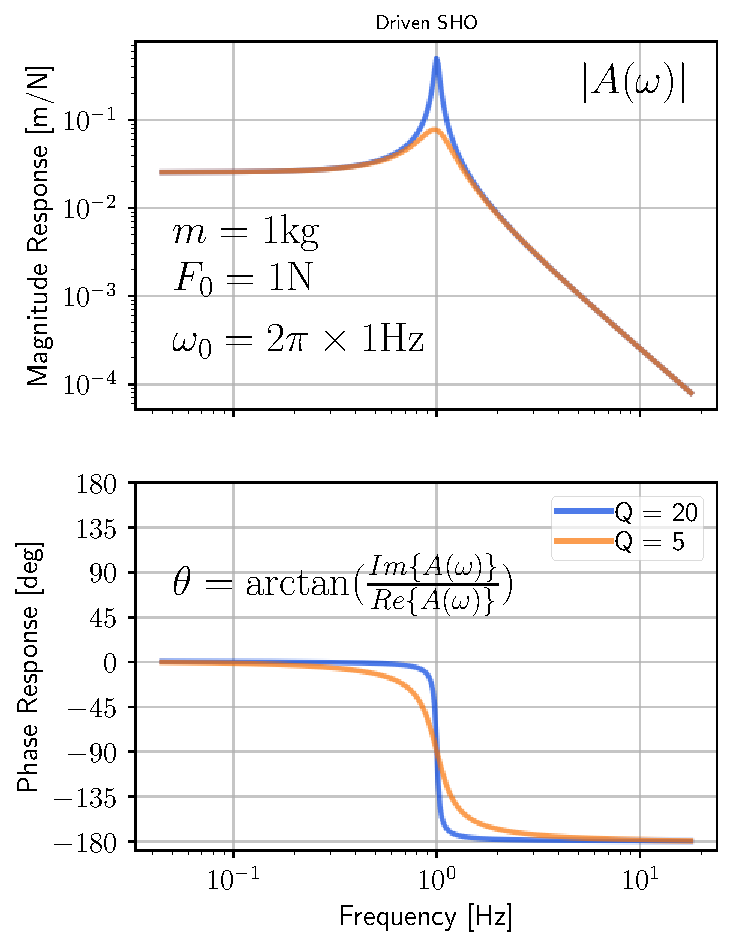
\includegraphics[width=0.8\textwidth]{DrivenSHO.pdf}

\end{column}
\end{columns}
%\pause
%DEMO: Air Track with magnets and \emph{lasers}.
\end{frame}



\begin{frame}
\frametitle{The Quality Factor: Estimation Test}

Fill in the missing parameters:
\begin{table}
\centering
    \resizebox{\columnwidth}{!}{%
    \begin{tabular}{|l|c|r|}
      \hline
    Item Name                     & Frequency (Hz)  & Quality Factor \\ \hline
    Rubber Stopper                       & 10       & 0.5      \\
    Church Bell (Cologne)                & 330      & 1500     \\
   Tuning Fork on Wood                   &         &          \\
   Mass on Track                         &         &          \\
   Mass on Track (w/ magnetic damping)   &         &          \\
  Suspension Bridges (e.g. Golden Gate)  &         &           \\
  Ionosphere (Schumann resonances)        & 8-30   & 3-5       \\
    Stop Sign (hit with a rubber mallet) & 200      & 1000     \\
    ${}_0S_0$ Dilational Mode of the Earth     & 0.0008   & 3000     \\
    75 mm silicon wafer                  & 800      & 50,000   \\
    Quartz Crystal Resonator             & 10$^6$   & $10^4$\,--\,$10^6$ \\
    Large, High Purity Glass             & 3000     & 10$^8$   \\ \hline
    \end{tabular}}
\end{table}

\end{frame}

\subsection{Resonance}
\begin{frame}
\frametitle{Examples of Resonance}
\begin{itemize}
\pause
\item Wine glass: thin walls, high Q (can be shattered by roosters ?)
\pause
\item Bridges: \href{https://en.wikipedia.org/wiki/Tacoma_Narrows_Bridge_(1940)}{Tacoma
    Narrows} ? (see video)
\pause
\item Ionospheric Resonances (driven by lightning and solar activity)
\pause
\item others?
\end{itemize}
\end{frame}

\begin{frame}
\frametitle{Schumann Resonances}
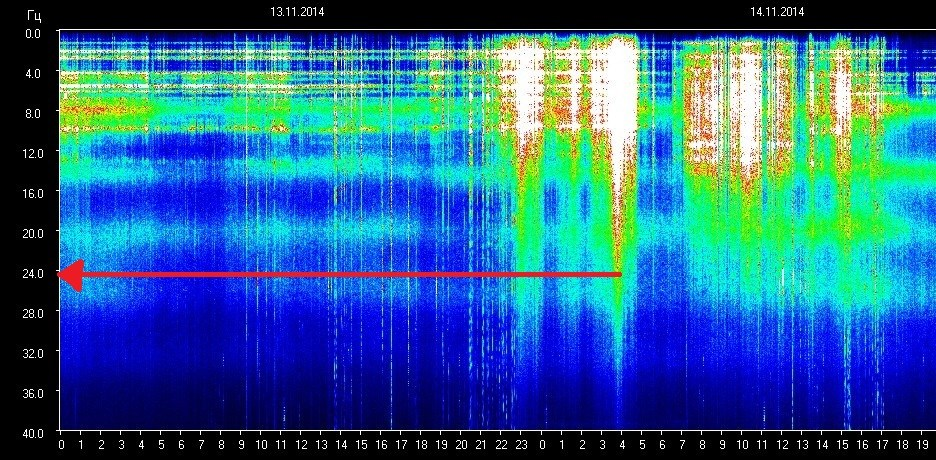
\includegraphics[width=\textwidth]{Schumann.jpg}
\end{frame}


\section{Energy of Oscillators}
\begin{frame}
\frametitle{Kinetic and Potential Energy}
\pause
\begin{enumerate}
\item total energy, $E =  \frac{1}{2} m v^2 + \frac{1}{2}k x^2$
\pause
\item for an undamped oscillator, the energy is
  conserved. $\frac{1}{2} k A^2$, where $A$ is the amplitude of the
  sinusoidal motion.
\end{enumerate}

\end{frame}

\begin{frame}
\frametitle{Resonant Ampification}
How much amplification do we get from a resonant system?
\pause
\begin{enumerate}
\item For a usual free mass, driven sinusoidally, $F = m a \implies x = - (F_0/m) / \omega^2$
\pause
\item For a resonant mass-spring, we have instead: $A =
  \frac{F_0/m}{\omega_0^2 + i \omega \frac{b}{m} - \omega^2}$
\pause
\item At the resonant frequency, $\omega = \omega_0$, so $A =
  \frac{F_0/m}{i \omega \frac{b}{m}}$ or, substituting our expression
  for Q,...
\pause
\item we see the amplification factor is just $Q$:  $A = -i Q \frac{F_0/m}{w_0^2}$

\end{enumerate}

\end{frame}



%\section{The Drag Force as Damping}
%\begin{frame}
%\frametitle{A Model for Drag Force}
%\end{frame}




\section{Summary}
\begin{frame}
\frametitle{Summary}
\begin{enumerate}
\pause
\item For linear systems, the resultant of two vibrations is just their sum.
\pause
\item Sum of two oscillations with different frequencies leads to \emph{beats}.
\pause
\item In a conservative system, the energy relations determine the
  motions.
%\item Drag force
\end{enumerate}
\end{frame}


\end{document}

